% Hasil
\section{Hasil}

\subsection{Perbandingan Statistik Deskriptif Sampel dan Parameter Nasional Tidak Resmi}

\begin{table}[H]
    \centering
    \caption{Perbandingan Statistik Deskriptif Sampel ($N=1.886$) dan Parameter Nasional Tidak Resmi per Subtes}
    \label{tab:deskriptif}
    \begin{spacing}{1.0}
    \begin{tabular}{lcccccc}
        \toprule
        Subtes & $M$ (Sampel) & $SD$ (Sampel) & $M$ (Nasional) & $SD$ (Nasional) & $\Delta M$ & $\Delta SD$ \\
        \midrule
        PU              & 633,26 & 76,85 & 500,00 & 71,52 & 133,26 & 5,33 \\
        PPU             & 669,96 & 61,50 & 500,00 & 100,00 & 169,96 & -38,50 \\
        PBM             & 680,95 & 76,62 & 500,00 & 100,00 & 180,95 & -23,38 \\
        PK              & 678,53 & 131,90 & 500,00 & 100,00 & 178,53 & 31,90 \\
        LBI Saintek     & 631,63 & 82,31 & 500,00 & 100,00 & 131,63 & -17,69 \\
        LBI Soshum      & 634,69 & 70,11 & 500,00 & 100,00 & 134,69 & -29,89 \\
        LBE             & 680,44 & 86,50 & 500,00 & 100,00 & 180,44 & -13,50 \\
        PM              & 653,23 & 100,01 & 500,00 & 100,00 & 153,23 & 0,01 \\
        \bottomrule
    \end{tabular}
    \end{spacing}
    \vspace{2mm}
    \begin{flushleft}
    \footnotesize\textit{Catatan.} $\Delta M = M_{\text{sampel}} - M_{\text{nasional}}$; $\Delta SD = SD_{\text{sampel}} - SD_{\text{nasional}}$. Parameter nasional tidak resmi bersumber dari tabel internal Panitia Seleksi Nasional Penerimaan Mahasiswa Baru (SNPMB) yang beredar di media sosial dan belum terverifikasi secara resmi (triangulasi parsial pada nilai maksimum PK dan PM; lihat Bagian Metode).
    \end{flushleft}
\end{table}


Rerata sampel melampaui rerata nasional sebesar 131,63--180,95 poin pada seluruh subtes (Tabel~\ref{tab:deskriptif}), sehingga sampel ($N=1.886$) condong ke skor tinggi. $SD$ sampel menyusut pada enam dari delapan subtes dibandingkan parameter nasional tidak resmi, dan penyusutan itu mengindikasikan \textit{restriction of range}. Penurunan terbesar teramati pada PPU ($-38,50$ poin) dan LBI Soshum ($-29,89$ poin). Sebaliknya, $SD$ PK membesar 31,90 poin akibat nilai ekstrem sebesar 1.173,55 (dievaluasi pada Subbagian Evaluasi Asumsi Distribusi). Selain itu, hanya 0,42\% sampel yang berada di bawah rerata nasional ($M=500$), jauh dari proporsi 50\% yang diharapkan pada sampel representatif.

\subsection{Evaluasi Asumsi Distribusi}
Tujuh statistik nasional tidak resmi per subtes menunjukkan bahwa distribusi skor menyimpang dari normal (Tabel~\ref{tab:nonnormal_diag}). Skor minimum nasional jauh lebih dekat ke rerata daripada yang diharapkan. Nilai $z$ minimum berkisar dari $-1,43$ (PK) hingga $-2,89$ (LBI Soshum), padahal pada populasi normal berukuran 846.518 peserta hadir minimum diharapkan sekitar $-4,72$ $SD$. Bila distribusi normal, jumlah peserta yang seharusnya berada di bawah minimum nasional berkisar dari sekitar 1.654 (LBI Soshum) hingga 64.760 (PK), sedangkan jumlah teramati sekitar satu. Skor $M - 3\,SD$ berada di bawah minimum nasional pada seluruh subtes. Di sisi atas, $z$ maksimum melampaui batas normal ($4,72$) pada PU ($5,51$), PM ($4,98$), dan PK ($6,74$, skor $1.173,55$), tetapi tidak pada subtes lain ($3,91$ pada LBE hingga $4,54$ pada LBI Saintek). Selisih rerata dan median bernilai positif pada enam subtes (PK $25,1$; LBE $16,3$; PM $10,9$) dan sedikit negatif pada kedua skor LBI ($-3,76$ dan $-3,65$). Kemiringan Bowley terbesar teramati pada PK ($0,26$), sedangkan rasio $\frac{IQR}{SD}$ ($1,33$--$1,54$) berada di sekitar nilai normal ($1,349$). Pola ini berupa distribusi miring ke kanan dengan ekor kiri terpotong dan paling menonjol pada PK, LBE, dan PM.

\begin{table}[H]
    \centering
    \caption{Diagnostik Nonnormalitas Parameter Nasional Tidak Resmi per Subtes}
    \label{tab:nonnormal_diag}
    \begin{spacing}{1.0}
    \resizebox{\textwidth}{!}{%
    \begin{tabular}{lcccccc}
        \toprule
        Subtes & $z$ Minimum & $z$ Maksimum & $N$ Diharapkan $<$ Minimum & Bowley & Rerata$-$Median & $\frac{IQR}{SD}$ \\
        \midrule
        PU & -2,71 & 5,51 & 2.826 & 0,04 & 5,4 & 1,33 \\
        PPU & -2,68 & 4,35 & 3.109 & 0,06 & 4,9 & 1,45 \\
        PBM & -2,70 & 4,41 & 2.917 & 0,03 & 4,9 & 1,39 \\
        PK & -1,43 & 6,74 & 64.760 & 0,26 & 25,1 & 1,36 \\
        LBI Saintek & -2,54 & 4,54 & 4.704 & -0,06 & -3,8 & 1,45 \\
        LBI Soshum & -2,89 & 4,17 & 1.654 & -0,04 & -3,6 & 1,43 \\
        LBE & -1,83 & 3,91 & 28.572 & 0,12 & 16,3 & 1,37 \\
        PM & -2,33 & 4,98 & 8.361 & 0,12 & 10,9 & 1,54 \\
        \bottomrule
    \end{tabular}%
    }
    \end{spacing}
    \vspace{2mm}
    \begin{flushleft}
    \footnotesize\textit{Catatan.} $z = \frac{\text{skor} - 500}{SD}$ nasional. Pada distribusi normal dengan $N_{\text{nasional}} = 846.518$, minimum dan maksimum diharapkan sekitar $\mp 4,72$ $SD$ dari rerata; kemiringan Bowley $= 0$; dan $\frac{IQR}{SD} = 1{,}349$, dengan $IQR$ sebagai rentang antarkuartil. ``$N$ Diharapkan $<$ Minimum'' = $N_{\text{nasional}} \cdot \Phi(z_{\min})$, yaitu jumlah peserta yang seharusnya berada di bawah minimum nasional bila distribusi normal (nilai teramati sekitar satu). Skor $M - 3\,SD$ berada di bawah minimum nasional pada seluruh subtes.
    \end{flushleft}
\end{table}


Dampak ketidaknormalan diperiksa melalui simulasi (Tabel~\ref{tab:nonnormal_sim}). Distribusi Johnson SB \autocite{johnson1949} untuk tiap subtes cocok dengan kuantil, rerata, dan $SD$ nasional (nilai fungsi tujuan $\leq 0,009$ pada semua subtes; galat kuantil umumnya di bawah tiga poin, terbesar $7,5$ poin pada median LBI Saintek, sedangkan galat rerata hingga $5,2$ poin dan galat $SD$ hingga $5,5$ poin). Skor komposit simulasi miring ke kanan (\textit{skewness} $0,41$--$0,42$; ekskurtosis berlebih $0,06$). Simulasi A (korelasi laten $0,425$) menghasilkan $SD$ skor komposit $68,3$, sedangkan simulasi B (korelasi laten $0,415$) menghasilkan $S_Z = 67,72$. Kedua simulasi menghasilkan pola yang sama. Di sekitar $\pm 1\,SD$, hasil simulasi dekat dengan normal (selisih skor kurang dari $1,5$ poin). Di ekor atas, peluang melampaui $M + 2\,S_Z$ adalah $3,44\%$ (A) dan $3,32\%$ (B) dibandingkan $2,28\%$ pada normal, dan peluang melampaui $M + 3\,S_Z$ adalah $0,407\%$ dan $0,380\%$ dibandingkan $0,135\%$. Peringkat nasional setara $M + 3\,S_Z$ berubah dari sekitar 1.143 menjadi 3.216--3.446. Skor komposit pada persentil normal ke-97,7 dan ke-99,9 pada simulasi B adalah $649$ dan $730$, atau $13,4$ dan $26,9$ poin di atas versi normal ($635$ dan $703$). Di ekor bawah, peluang berada di bawah $M - 2\,S_Z$ hanya $0,89\%$ (A) dan $0,83\%$ (B) dibandingkan $2,28\%$, dan peluang di bawah $M - 3\,S_Z$ praktis nol. Skor pada persentil normal ke-2,3 dan ke-0,13 pada simulasi B adalah $381$ dan $343$ dibandingkan $365$ dan $297$.

\begin{table}[H]
    \centering
    \caption{Sensitivitas Persentil dan Skor Komposit terhadap Asumsi Normal dengan Marginal Johnson SB dan \textit{Copula} Gaussian}
    \label{tab:nonnormal_sim}
    \begin{spacing}{1.0}
    \resizebox{\textwidth}{!}{%
    \begin{tabular}{lccccccc}
        \toprule
        & \multicolumn{3}{c}{Peluang Ekor (\%)} & \multicolumn{4}{c}{Skor Komposit pada Persentil Normal} \\
        \cmidrule(lr){2-4} \cmidrule(lr){5-8}
        Titik & Normal & Simulasi A & Simulasi B & Normal & Simulasi A & Simulasi B & Selisih B \\
        \midrule
        $M - 3\,S_Z$ & 0,135 & $<0{,}001$ & $<0{,}001$ & 296,9 & 341,6 & 342,5 & 45,7 \\
        $M - 2\,S_Z$ & 2,275 & 0,891 & 0,834 & 364,6 & 380,2 & 381,1 & 16,5 \\
        $M - 1\,S_Z$ & 15,866 & 16,275 & 16,014 & 432,3 & 431,3 & 431,9 & -0,3 \\
        $M + 1\,S_Z$ & 15,866 & 16,297 & 16,108 & 567,7 & 569,1 & 568,5 & 0,8 \\
        $M + 2\,S_Z$ & 2,275 & 3,439 & 3,325 & 635,4 & 650,2 & 648,8 & 13,3 \\
        $M + 3\,S_Z$ & 0,135 & 0,407 & 0,380 & 703,1 & 732,3 & 730,1 & 26,9 \\
        \bottomrule
    \end{tabular}%
    }
    \end{spacing}
    \vspace{2mm}
    \begin{flushleft}
    \footnotesize\textit{Catatan.} Skor komposit adalah rerata delapan subtes, dengan 1.000.000 peserta virtual. Marginal tiap subtes dihampiri distribusi Johnson SB yang dicocokkan ke kuantil, rerata, dan $SD$ nasional tidak resmi, dan dependensi dimodelkan dengan \textit{copula} Gaussian berkorelasi seragam. Simulasi A memakai korelasi laten $= 0,425$ ($\bar{R}$ Thorndike) dan menghasilkan $SD$ skor komposit $= 68,3$. Simulasi B memakai korelasi laten $= 0,415$, dikalibrasi agar $SD$ skor komposit $= S_Z = 67,72$. Skor komposit simulasi dipusatkan ke rerata $500$ (pergeseran 2,39 poin). Titik $M \pm k\,S_Z$ dengan $M = 500$. Peluang ekor mengacu pada sisi bawah untuk $k<0$ dan sisi atas untuk $k>0$. Selisih B = skor simulasi B $-$ skor normal.
    \end{flushleft}
\end{table}


Estimasi korelasi dan translasi persentil pada Tabel~\ref{tab:ranking_subtes} dan~\ref{tab:ranking_komposit} tetap menggunakan pendekatan normal sebagai model kerja. Simulasi menunjukkan arah dan kisaran ukuran dampaknya, terutama di ekor distribusi.

\subsection{Estimasi Korelasi Antarsubtes}
Estimasi korelasi Pearson antardelapan subtes berdasarkan data sampel ($N=1.886$) menghasilkan rerata korelasi \textit{off-diagonal} sebesar 0,300 (Tabel~\ref{tab:korelasi}, Gambar~\ref{fig:heatmap_raw}).

\begin{table}[H]
    \centering
    \caption{Matriks Korelasi Pearson Antarsubtes (Data Sampel, $N=1.886$)}
    \label{tab:korelasi}
    \begin{spacing}{1.0}
    \resizebox{\textwidth}{!}{%
    \begin{tabular}{lcccccccc}
        \toprule
        & PU & PPU & PBM & PK & LBI Saintek & LBI Soshum & LBE & PM \\
        \midrule
        PU           & 1,000 & 0,362 & 0,388 & 0,451 & 0,315 & 0,240 & 0,402 & 0,380 \\
        PPU          & 0,362 & 1,000 & 0,420 & 0,277 & 0,248 & 0,214 & 0,383 & 0,279 \\
        PBM          & 0,388 & 0,420 & 1,000 & 0,325 & 0,273 & 0,198 & 0,376 & 0,277 \\
        PK           & 0,451 & 0,277 & 0,325 & 1,000 & 0,274 & 0,124 & 0,275 & 0,400 \\
        LBI Saintek  & 0,315 & 0,248 & 0,273 & 0,274 & 1,000 & 0,264 & 0,328 & 0,267 \\
        LBI Soshum   & 0,240 & 0,214 & 0,198 & 0,124 & 0,264 & 1,000 & 0,284 & 0,151 \\
        LBE          & 0,402 & 0,383 & 0,376 & 0,275 & 0,328 & 0,284 & 1,000 & 0,236 \\
        PM           & 0,380 & 0,279 & 0,277 & 0,400 & 0,267 & 0,151 & 0,236 & 1,000 \\
        \bottomrule
    \end{tabular}%
    }
    \end{spacing}
    \vspace{2mm}
    \begin{flushleft}
    \footnotesize\textit{Catatan.} Rerata korelasi \textit{off-diagonal} (28 pasangan unik) $\approx 0,300$.
    \end{flushleft}
\end{table}


\begin{figure}[H]
    \centering
    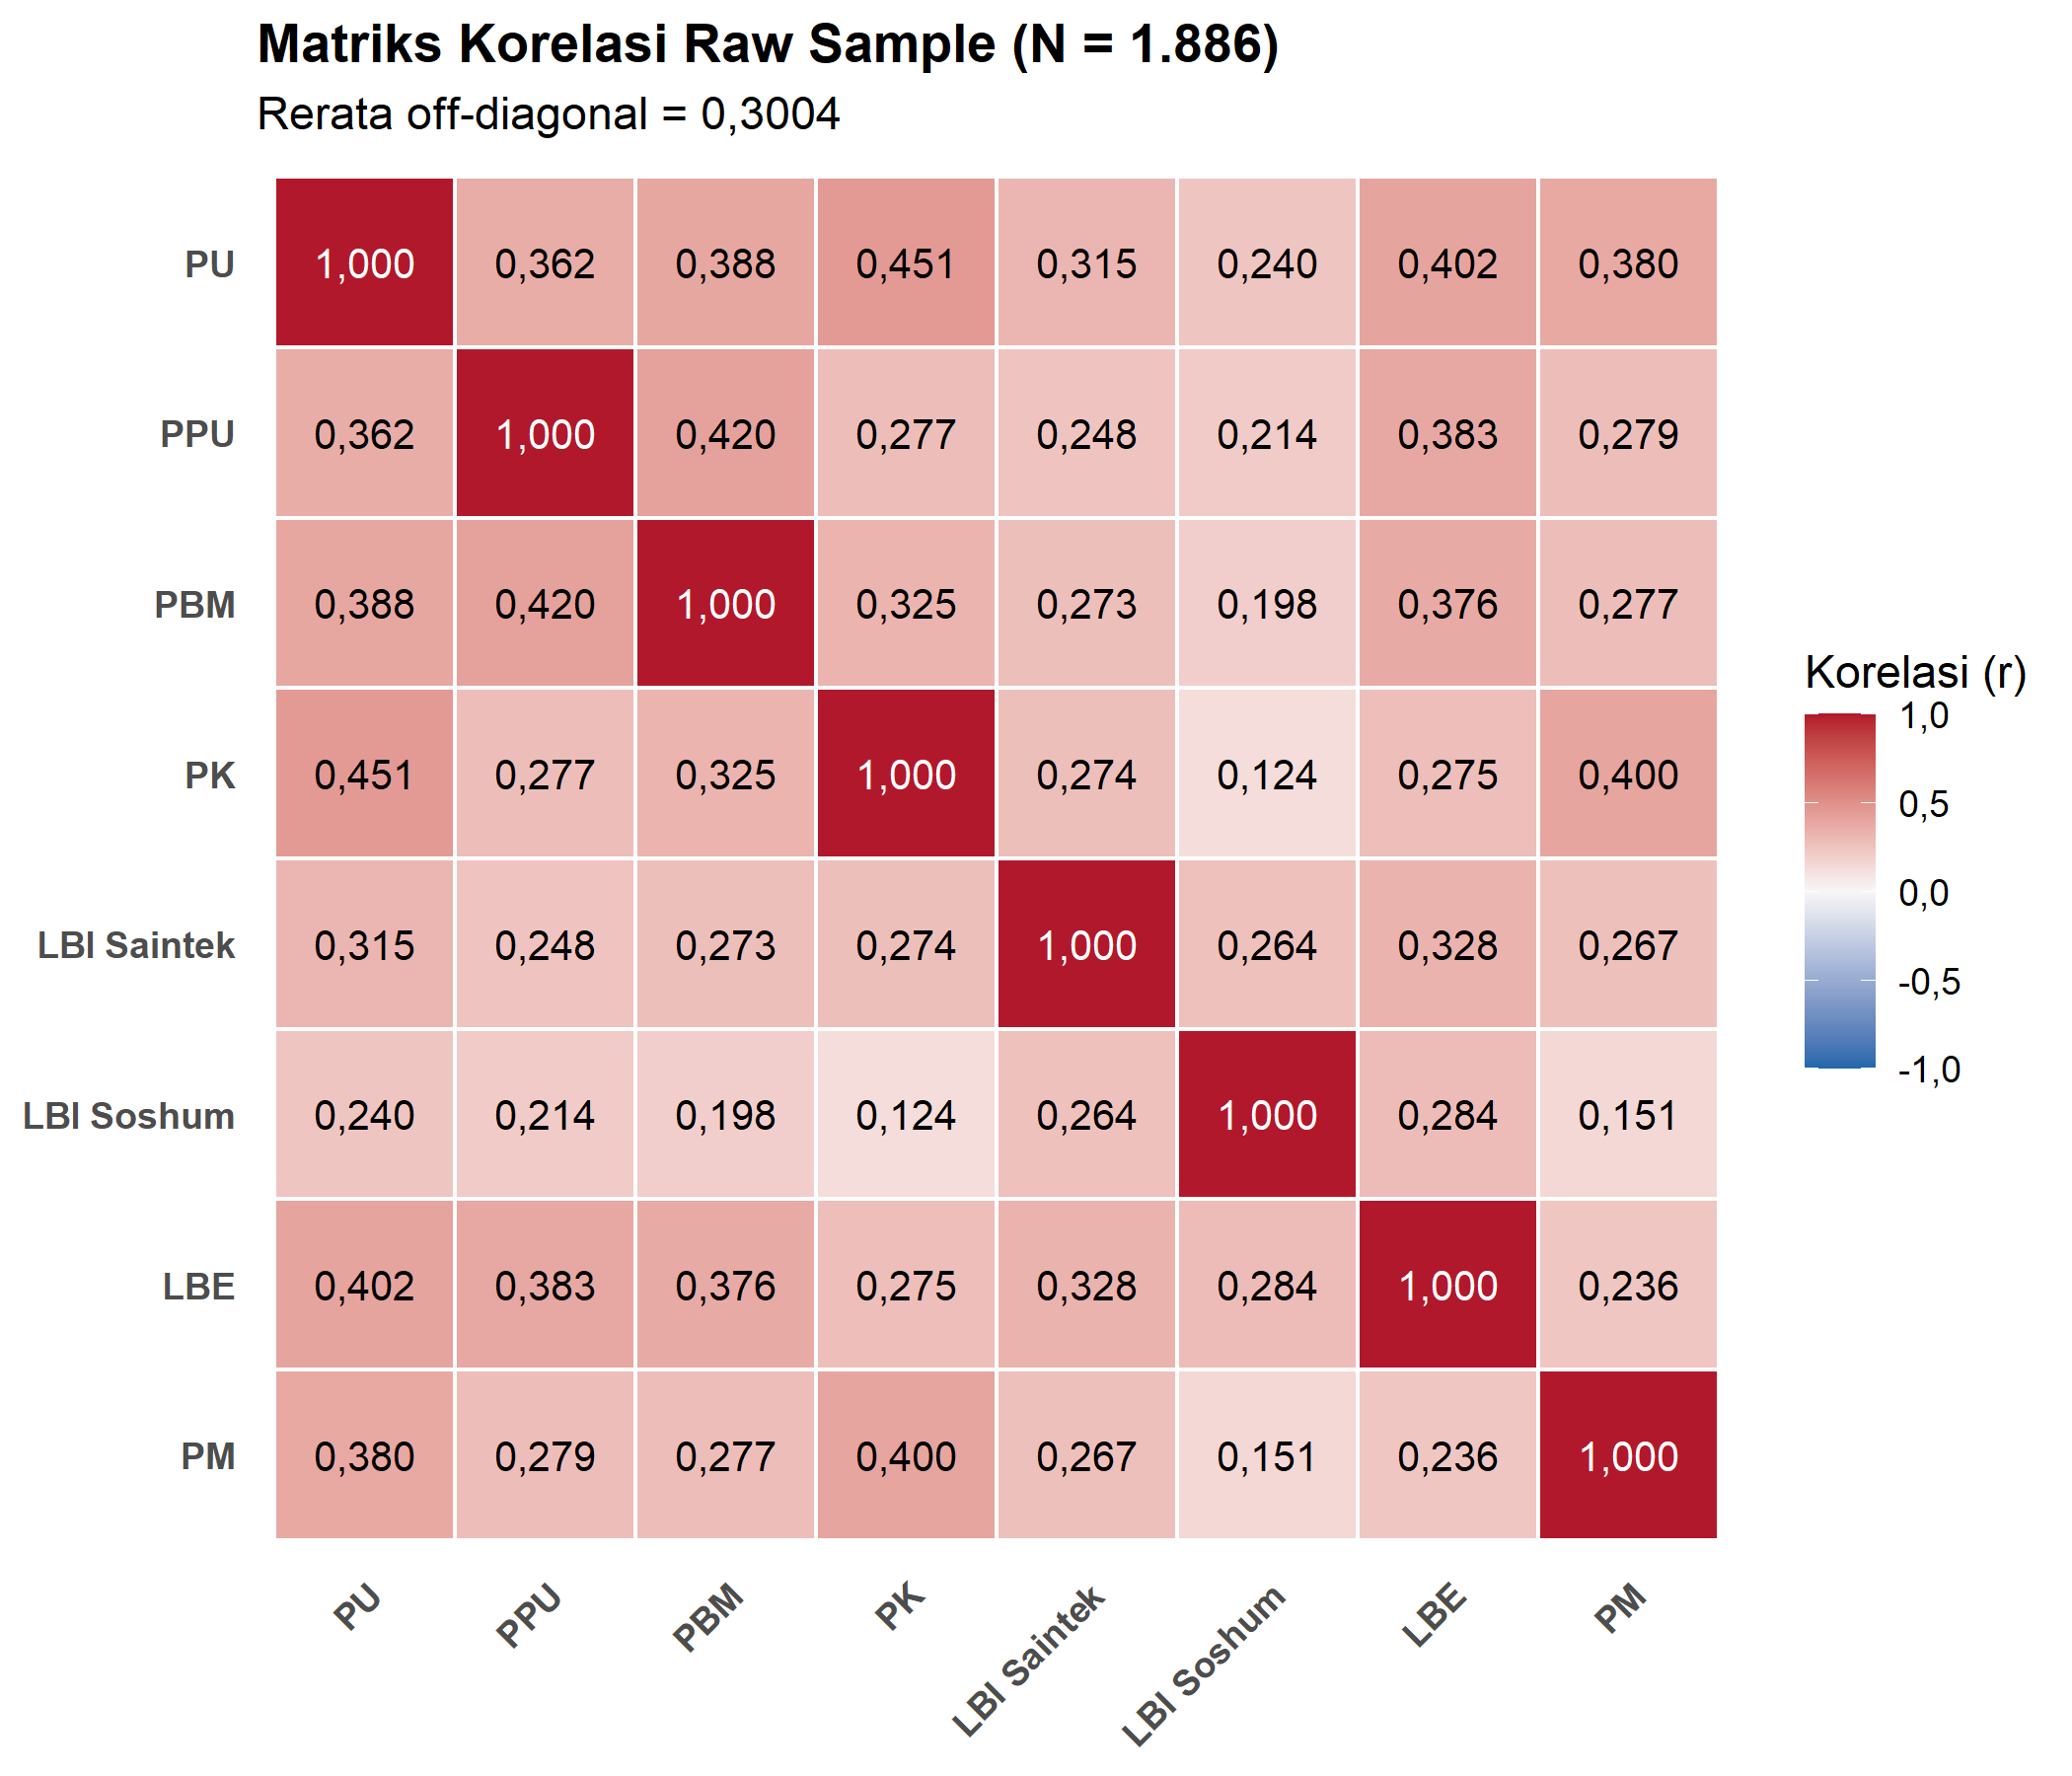
\includegraphics[width=0.65\textwidth]{../output/figures/heatmap_raw.png}
    \caption{\textit{Heatmap} Matriks Korelasi Pearson Antarsubtes (Data Sampel, $N=1.886$)}
    \label{fig:heatmap_raw}
\end{figure}

\subsection{Koreksi Kuantitatif \textit{Restriction of Range} (Thorndike Case III)}
Koreksi Thorndike Case III dengan $S_Z \approx 67,72$, hasil iterasi titik tetap, menghasilkan matriks korelasi terkoreksi dengan rerata \textit{off-diagonal} sebesar 0,425 (Tabel~\ref{tab:korelasi_terkoreksi}, Gambar~\ref{fig:heatmap_thorndike}).

\begin{table}[H]
    \centering
    \caption{Matriks Korelasi Antarsubtes Terkoreksi \textit{Restriction of Range} (Thorndike Case III)}
    \label{tab:korelasi_terkoreksi}
    \begin{spacing}{1.0}
    \resizebox{\textwidth}{!}{%
    \begin{tabular}{lcccccccc}
        \toprule
        & PU & PPU & PBM & PK & LBI Saintek & LBI Soshum & LBE & PM \\
        \midrule
        PU           & 1,000 & 0,485 & 0,514 & 0,575 & 0,447 & 0,354 & 0,527 & 0,508 \\
        PPU          & 0,485 & 1,000 & 0,523 & 0,417 & 0,374 & 0,318 & 0,494 & 0,407 \\
        PBM          & 0,514 & 0,523 & 1,000 & 0,464 & 0,401 & 0,310 & 0,495 & 0,413 \\
        PK           & 0,575 & 0,417 & 0,464 & 1,000 & 0,413 & 0,258 & 0,426 & 0,524 \\
        LBI Saintek  & 0,447 & 0,374 & 0,401 & 0,413 & 1,000 & 0,361 & 0,448 & 0,397 \\
        LBI Soshum   & 0,354 & 0,318 & 0,310 & 0,258 & 0,361 & 1,000 & 0,385 & 0,270 \\
        LBE          & 0,527 & 0,494 & 0,495 & 0,426 & 0,448 & 0,385 & 1,000 & 0,382 \\
        PM           & 0,508 & 0,407 & 0,413 & 0,524 & 0,397 & 0,270 & 0,382 & 1,000 \\
        \bottomrule
    \end{tabular}%
    }
    \end{spacing}
    \vspace{2mm}
    \begin{flushleft}
    \footnotesize\textit{Catatan.} Rerata korelasi \textit{off-diagonal} terkoreksi $\approx 0,425$.
    \end{flushleft}
\end{table}


\begin{figure}[H]
    \centering
    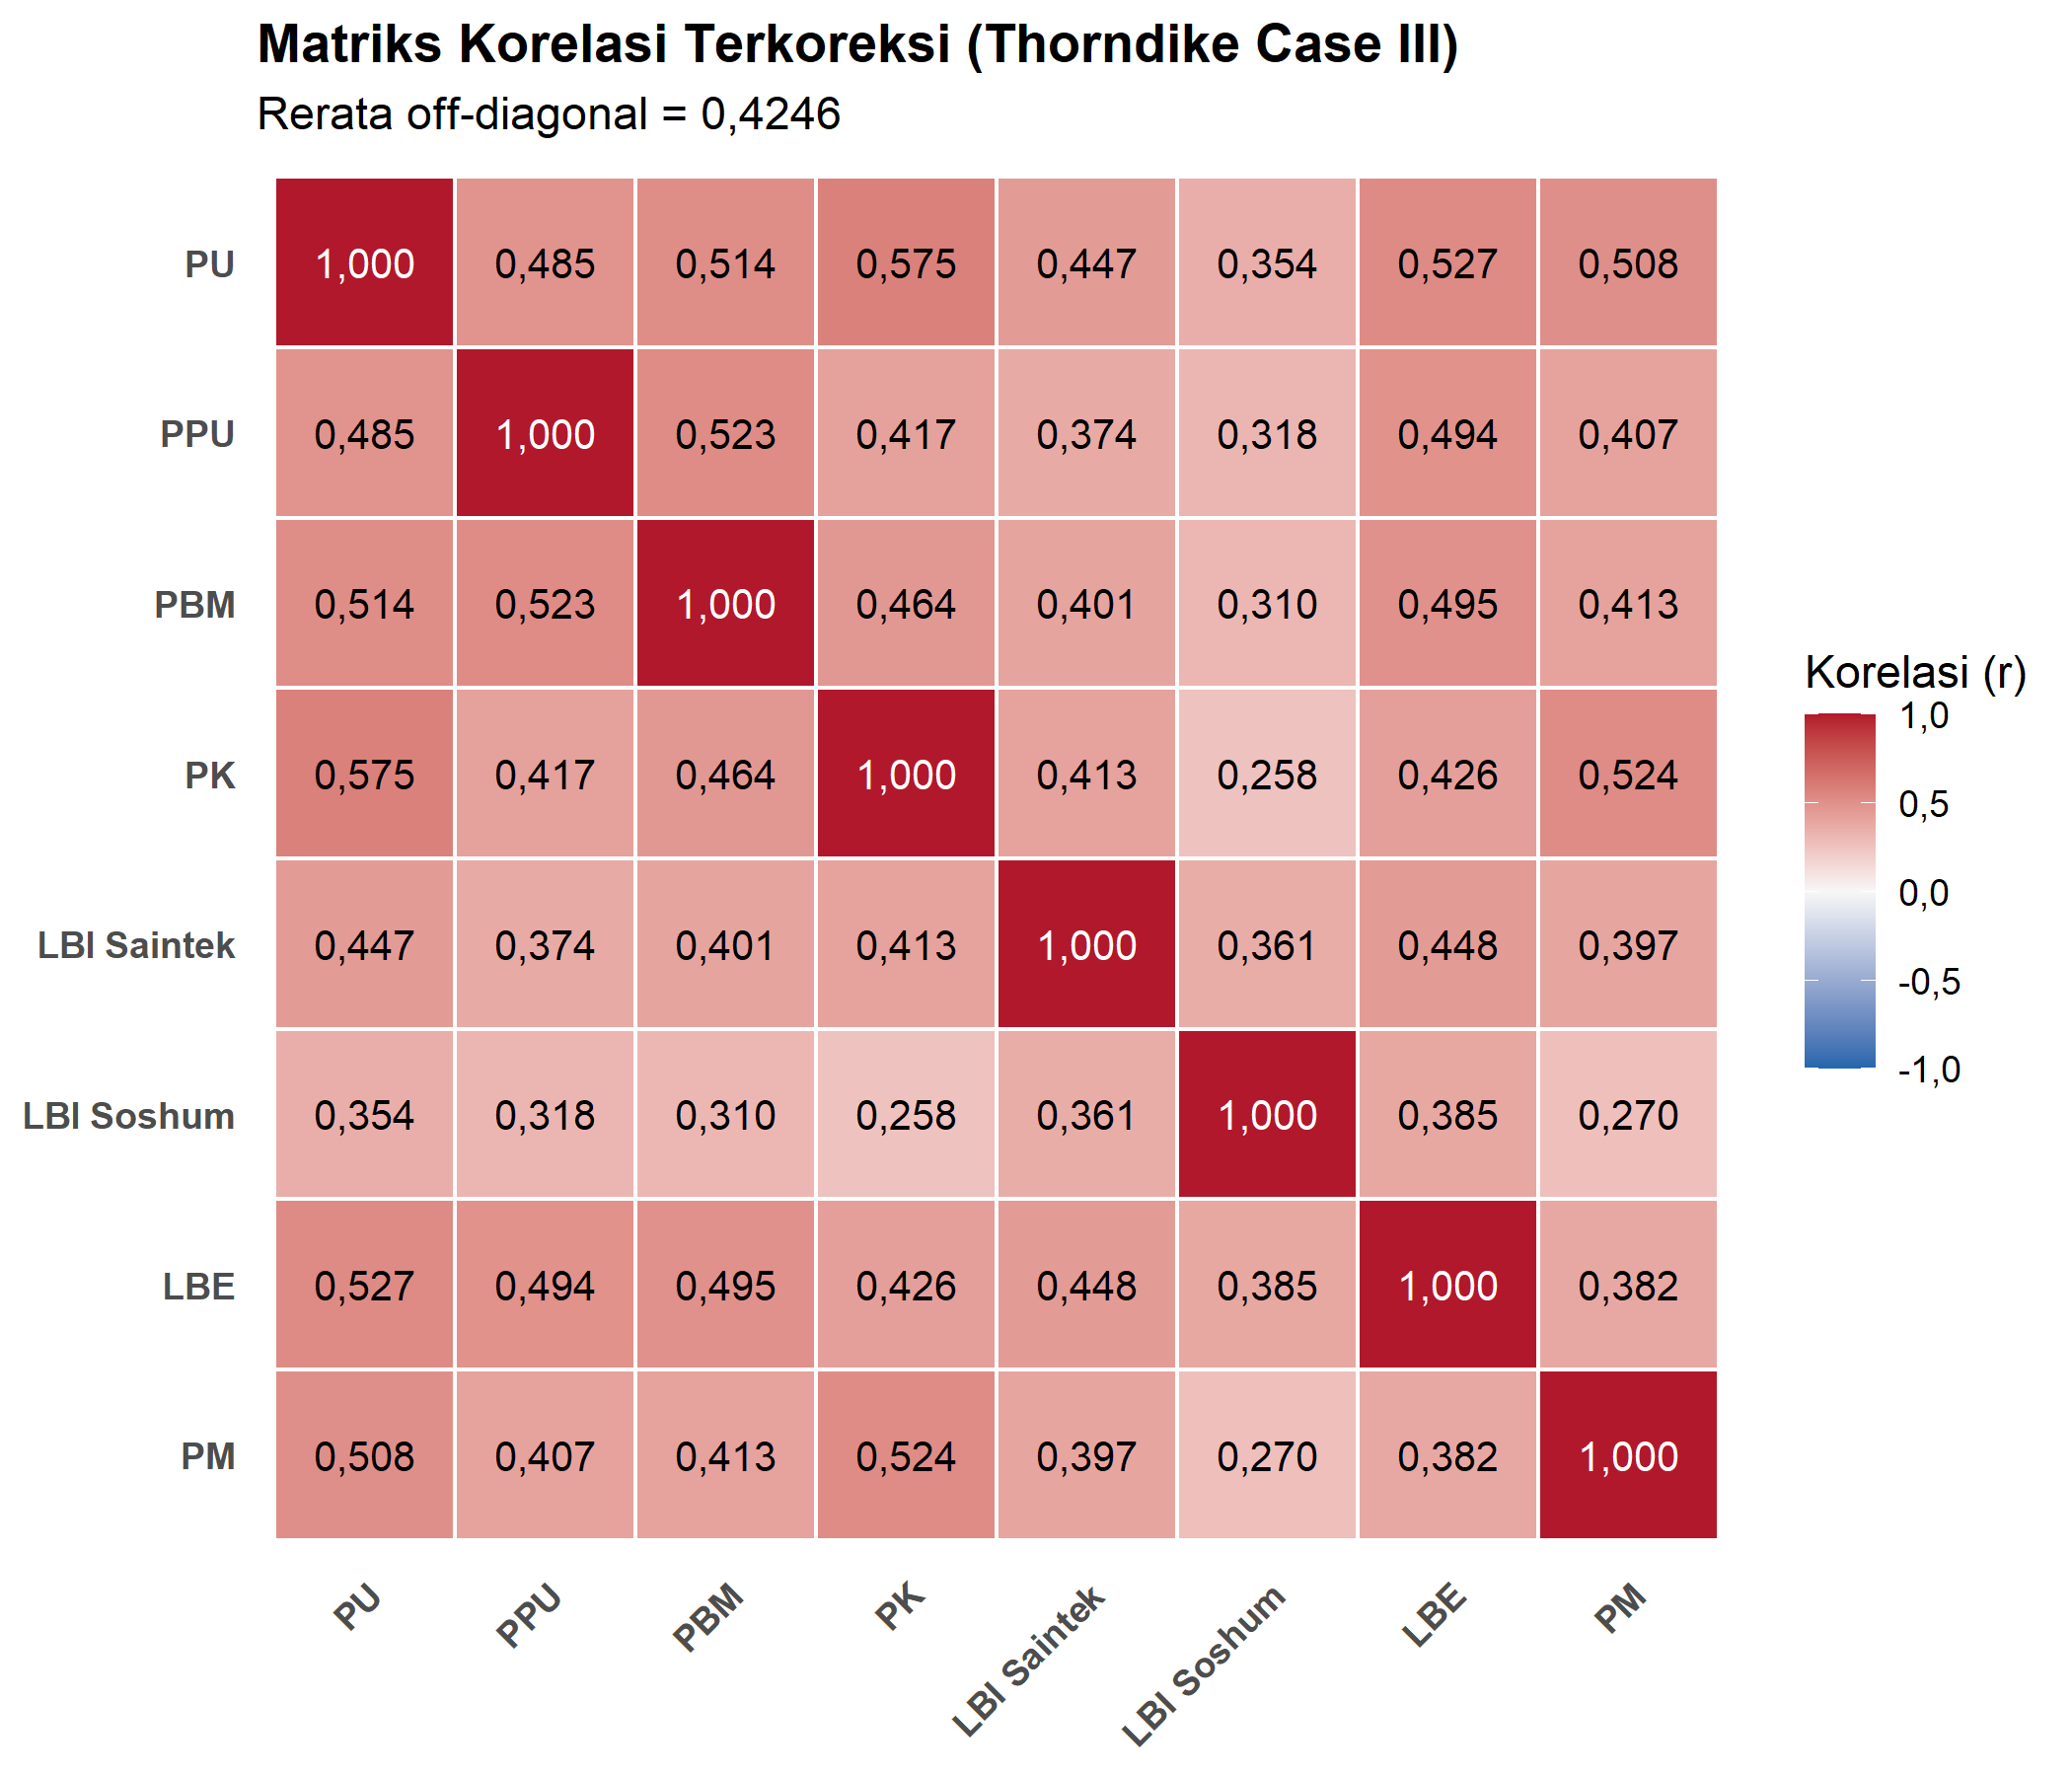
\includegraphics[width=0.65\textwidth]{../output/figures/heatmap_thorndike.png}
    \caption{\textit{Heatmap} Matriks Korelasi Antarsubtes Terkoreksi \textit{Restriction of Range} (Thorndike Case III)}
    \label{fig:heatmap_thorndike}
\end{figure}

\subsection{Analisis Faktor Eksploratori dan Konfirmatori}
Model 2 (dua faktor berkorelasi, Literasi dan Numerasi) memiliki kecocokan yang lebih baik secara signifikan dibandingkan Model 1 (\textit{g-factor} tunggal) (Tabel~\ref{tab:cfa_fit}, Gambar~\ref{fig:scree_parallel}). CFI meningkat dari $0,932$ menjadi $0,967$, RMSEA menurun dari $0,073$ menjadi $0,052$, dan uji selisih $\chi^2$ berskala Satorra--Bentler signifikan ($\Delta\chi^2(1) = 91,55$, $p < 0,001$). AIC Model 2 juga lebih rendah ($173.536,4$ berbanding $173.638,9$), sehingga Model 2 unggul pada seluruh kriteria kecocokan yang diuji.

\begin{table}[H]
    \centering
    \caption{Perbandingan Indeks Kecocokan Model 1 (\textit{g-factor} Tunggal) dan Model 2 (Dua Faktor Berkorelasi) pada CFA}
    \label{tab:cfa_fit}
    \begin{spacing}{1.0}
    \resizebox{\textwidth}{!}{%
    \begin{tabular}{lcccccccc}
        \toprule
        Model & $\chi^2_{\text{SB}}$ & $df$ & CFI & TLI & RMSEA [90\% CI] & SRMR & AIC & $\Delta\chi^2$ ($df$) \\
        \midrule
        Model 1: 1-Faktor (g-General)    & 220,17 & 20 & 0,932 & 0,904 & 0,073 [0,065; 0,082] & 0,042 & 173638,9 & - \\
        Model 2: 2-Faktor (Literasi vs Numerasi) & 117,26 & 19 & 0,967 & 0,951 & 0,052 [0,044; 0,062] & 0,031 & 173536,4 & 91,55 (1)$^{***}$ \\
        \bottomrule
    \end{tabular}%
    }
    \end{spacing}
    \vspace{2mm}
    \begin{flushleft}
    \footnotesize\textit{Catatan.} $N = 1.886$. Model 1 memuat \textit{g-factor} tunggal, sedangkan Model 2 memuat dua faktor berkorelasi (Literasi dan Numerasi). Estimator yang dipakai adalah \textit{robust maximum likelihood} (MLM). $\chi^2_{\text{SB}}$ adalah \textit{scaled chi-square} Satorra--Bentler; CFI = \textit{Comparative Fit Index}; TLI = \textit{Tucker--Lewis Index}; RMSEA = \textit{Root Mean Square Error of Approximation}; SRMR = \textit{Standardized Root Mean Square Residual}; AIC = \textit{Akaike Information Criterion}. Signifikansi $\Delta\chi^2$: $^{*}p < 0,05$; $^{**}p < 0,01$; $^{***}p < 0,001$ (dihitung dari nilai $p$ eksak).
    \end{flushleft}
\end{table}


\begin{figure}[H]
    \centering
    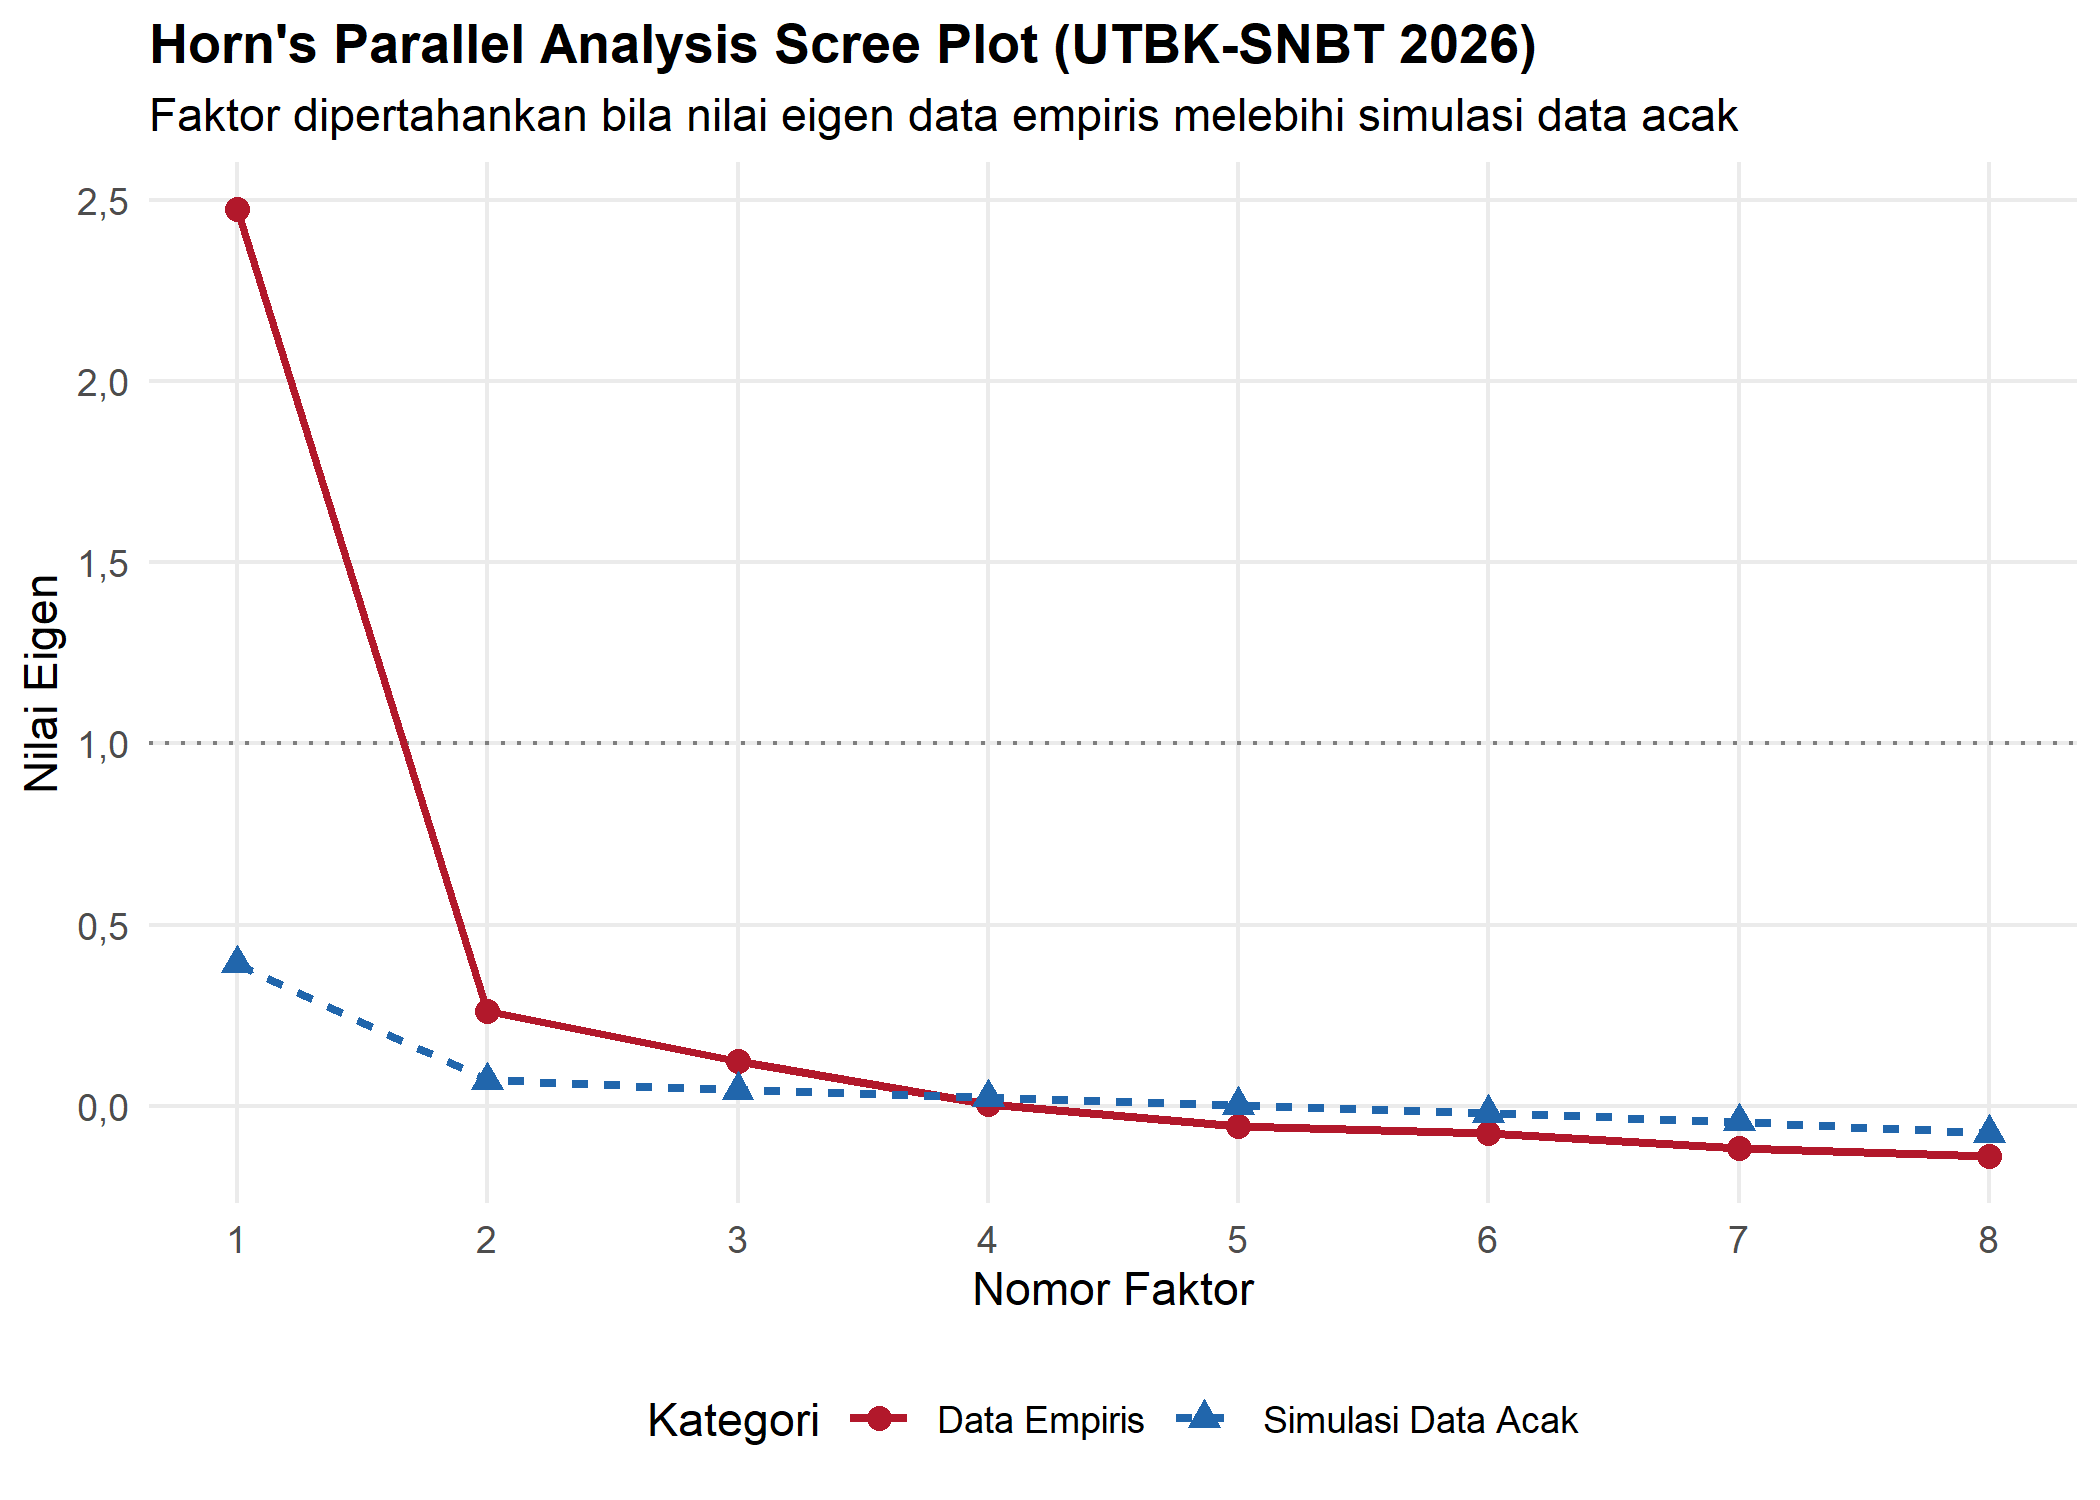
\includegraphics[width=0.65\textwidth]{../output/figures/scree_parallel_plot.png}
    \caption{\textit{Scree Plot} dan \textit{Horn's Parallel Analysis} untuk Diagnostik Retensi Faktor}
    \label{fig:scree_parallel}
\end{figure}

\textit{Parallel Analysis} berbasis faktor (Gambar~\ref{fig:scree_parallel}) menyarankan tiga faktor. Nilai eigen faktor-analitik teramati ke-1, ke-2, dan ke-3 ($2,473$; $0,261$; $0,122$) melampaui nilai eigen hasil simulasi data acak ($0,392$; $0,070$; $0,044$), sedangkan faktor ke-4 tidak ($0,006$ berbanding $0,023$). Jumlah ini berbeda dari struktur dua faktor yang ditetapkan apriori. Struktur dua faktor tetap dipertahankan karena tiga alasan: (1) pembedaan Literasi dan Numerasi bersandar pada kerangka teori yang dirumuskan sebelum analisis (lihat Tinjauan Pustaka); (2) nilai eigen faktor ketiga ($0,122$) jauh lebih kecil daripada faktor pertama ($2,473$) dan kedua ($0,261$), sehingga sumbangannya terhadap varians bersama relatif kecil; dan (3) pada sampel yang besar ($N = 1.886$), \textit{Parallel Analysis} dapat mengenali faktor kecil yang kurang bermakna secara substantif.

EFA tiga-faktor (rotasi \textit{oblimin}) menunjukkan bahwa faktor ketiga dibebani terutama oleh kedua skor LBI (LBI Soshum $0,523$; LBI Saintek $0,440$) dan sebagian oleh LBE ($0,322$). Dua faktor lainnya berisi subtes kuantitatif (PK $0,747$; PM $0,516$; PU $0,433$) dan subtes literasi umum (PPU $0,675$; PBM $0,595$; LBE $0,384$). Pola ini konsisten dengan tafsiran bahwa faktor ketiga mencerminkan varians bersama dua skor yang berasal dari satu tes LBI. Faktor itu hanya dibebani dua indikator utama, dan tafsiran ini belum diuji pada data independen. Pengaruh dependensi LBI terhadap hasil utama diperiksa pada Subbagian Sensitivitas terhadap Perlakuan Dua Skor LBI.

Sebagai pembanding, EFA dua-faktor dengan rotasi \textit{oblimin} menghasilkan kecocokan yang baik (CFI $= 0,982$; RMSEA $= 0,046$) dengan korelasi antarfaktor sebesar $0,635$, lebih rendah daripada $\phi = 0,813$ pada CFA. Selisih ini kemungkinan terkait dengan batasan nol pada \textit{cross-loading} (muatan subtes pada faktor di luar faktor utamanya) dalam model CFA. Batasan itu berpengaruh terutama pada PU, yang pada EFA membebani kedua faktor (indeks kompleksitas $1,95$, ukuran banyaknya faktor yang dimuati satu subtes). Dengan demikian, nilai $\phi$ pada CFA bergantung pada spesifikasi struktur sederhana (setiap subtes hanya memuat satu faktor).

Muatan faktor terstandarisasi pada Model 2 (Tabel~\ref{tab:factor_loadings}) menunjukkan bahwa lima subtes literasi (PPU, PBM, LBI Saintek, LBI Soshum, LBE) membebani faktor Literasi dengan muatan berkisar $0,384$--$0,629$. Tiga subtes kuantitatif (PU, PK, PM) membebani faktor Numerasi dengan muatan $0,554$--$0,736$. Seluruh muatan signifikan secara statistik ($p < 0,001$). LBI Saintek dan LBI Soshum sama-sama membebani faktor Literasi, dengan muatan LBI Soshum ($0,384$) lebih rendah daripada LBI Saintek ($0,498$). Korelasi antarfaktor laten tergolong tinggi ($\phi = 0,813$; $p < 0,001$). Meskipun Model 2 lebih unggul secara statistik, kedua faktor berbagi varians bersama yang substansial, sejalan dengan keberadaan \textit{g-factor} yang mendasari keduanya.

\begin{table}[H]
    \centering
    \caption{Muatan Faktor Terstandarisasi dan Komunalitas Subtes pada Model 2 (CFA)}
    \label{tab:factor_loadings}
    \begin{spacing}{1.0}
    \begin{tabular}{llcccc}
        \toprule
        Dimensi Laten & Subtes & $\lambda$ (Std.) & $SE$ & $z$ & $R^2$ ($h^2$) \\
        \midrule
        Literasi        & PPU          & 0,602$^{***}$ & 0,021 & 28,73 & 0,362 \\
        Literasi        & PBM          & 0,622$^{***}$ & 0,019 & 32,93 & 0,387 \\
        Literasi        & LBI Saintek  & 0,498$^{***}$ & 0,022 & 22,15 & 0,248 \\
        Literasi        & LBI Soshum   & 0,384$^{***}$ & 0,024 & 16,03 & 0,148 \\
        Literasi        & LBE          & 0,629$^{***}$ & 0,019 & 33,76 & 0,395 \\
        Numerasi        & PU           & 0,736$^{***}$ & 0,017 & 43,68 & 0,541 \\
        Numerasi        & PK           & 0,622$^{***}$ & 0,020 & 30,90 & 0,387 \\
        Numerasi        & PM           & 0,554$^{***}$ & 0,020 & 27,80 & 0,307 \\
        \bottomrule
    \end{tabular}
    \end{spacing}
    \vspace{2mm}
    \begin{flushleft}
    \footnotesize\textit{Catatan.} Bintang pada $\lambda$ menandakan signifikansi tiap muatan: $^{*}p < 0,05$; $^{**}p < 0,01$; $^{***}p < 0,001$. $SE$ = kesalahan standar; $z$ = nilai uji rasio kritis; $R^2$ ($h^2$) = proporsi varians yang dijelaskan oleh faktor laten terkait. Korelasi antarfaktor laten adalah $\phi = 0,813$$^{***}$.
    \end{flushleft}
\end{table}


\subsection{Sensitivitas terhadap Perlakuan Dua Skor LBI}
Pertama, model CFA dua-faktor diperluas dengan kovarians residual antara kedua skor LBI (Tabel~\ref{tab:sens_cfa}). Perluasan ini memperbaiki kecocokan model secara statistik ($\Delta\chi^2(1) = 17,3$, $p < 0,001$; CFI dari $0,967$ menjadi $0,973$; RMSEA dari $0,052$ menjadi $0,049$; AIC dan \textit{Bayesian Information Criterion} (BIC) menurun). Namun, korelasi residualnya kecil ($0,108$), korelasi antarfaktor hampir tidak berubah ($\phi$ dari $0,813$ menjadi $0,816$), dan muatan kedua LBI hanya bergeser sedikit (LBI Saintek dari $0,498$ menjadi $0,484$; LBI Soshum dari $0,384$ menjadi $0,365$). Dependensi antar-LBI signifikan secara statistik pada sampel sebesar ini, tetapi kecil secara praktis terhadap struktur dua-faktor.

\begin{table}[H]
    \centering
    \caption{Analisis Sensitivitas CFA Model Dua Faktor dengan dan tanpa Kovarians Residual antara LBI Saintek dan LBI Soshum}
    \label{tab:sens_cfa}
    \begin{spacing}{1.0}
    \resizebox{\textwidth}{!}{%
    \begin{tabular}{lcccccccccc}
        \toprule
        Model & $\chi^2_{\text{SB}}$ & $df$ & CFI & RMSEA & SRMR & AIC & BIC & $\phi$ & $r_{\text{resid}}$ & $\Delta\chi^2$ ($df$) \\
        \midrule
        Utama: 2-faktor & 117,3 & 19 & 0,967 & 0,052 & 0,031 & 173536 & 173631 & 0,813 & - & - \\
        2-faktor + kovarians residual LBI & 99,1 & 18 & 0,973 & 0,049 & 0,028 & 173520 & 173620 & 0,816 & 0,108 & 17,3 (1)$^{***}$ \\
        \bottomrule
    \end{tabular}%
    }
    \end{spacing}
    \vspace{2mm}
    \begin{flushleft}
    \footnotesize\textit{Catatan.} $N = 1.886$. Estimator yang dipakai adalah \textit{robust maximum likelihood} (MLM). Model utama identik dengan Model 2 pada Tabel~\ref{tab:cfa_fit}. $\phi$ = korelasi antarfaktor laten terstandar; $r_{\text{resid}}$ = korelasi residual terstandar antara LBI Saintek dan LBI Soshum. CFI = \textit{Comparative Fit Index}; RMSEA = \textit{Root Mean Square Error of Approximation}; SRMR = \textit{Standardized Root Mean Square Residual}; AIC = \textit{Akaike Information Criterion}; BIC = \textit{Bayesian Information Criterion}. Signifikansi $\Delta\chi^2$: $^{*}p < 0,05$; $^{**}p < 0,01$; $^{***}p < 0,001$ (dihitung dari nilai $p$ eksak).
    \end{flushleft}
\end{table}


Kedua, koreksi Thorndike Case III diulang dengan salah satu atau kedua skor LBI dikeluarkan dari skor komposit (Tabel~\ref{tab:sens_thorndike}). Skor komposit dihitung ulang sebagai rerata subtes yang tersisa, dan tiap subtes memakai $SD$ nasional tidak resminya sendiri. Rerata korelasi terkoreksi tetap berada pada kisaran sempit, $0,414$--$0,425$, dan $S_Z$ pada $67,43$--$68,31$, dibandingkan $\bar{R} = 0,425$ dan $S_Z = 67,72$ pada spesifikasi utama. Pembobotan ganda LBI pada skor komposit delapan subtes ($\frac{2}{8}$) tidak menggeser estimasi utama secara berarti. Rasio $SD$ tersirat terhadap $SD$ nasional tidak resmi pada keempat skenario berkisar $0,645$--$1,498$, sehingga keterbatasan homogenitas pada subbagian berikut tidak bergantung pada perlakuan LBI.

\begin{table}[H]
    \centering
    \caption{Analisis Sensitivitas Thorndike Case III terhadap Perlakuan LBI pada Skor Komposit}
    \label{tab:sens_thorndike}
    \begin{spacing}{1.0}
    \resizebox{\textwidth}{!}{%
    \begin{tabular}{lccccccc}
        \toprule
        Skenario & $k$ & $\bar{r}$ \textit{Raw Sample} & $s_Z$ Sampel & $S_Z$ Populasi & $\lambda^2$ & $\bar{R}$ Terkoreksi & Rasio $SD$ (min--maks) \\
        \midrule
        8 subtes (spesifikasi utama) & 8 & 0,300 & 53,84 & 67,72 & 0,582 & 0,425 & 0,674--1,498 \\
        7 subtes tanpa LBI Soshum & 7 & 0,330 & 57,71 & 68,03 & 0,390 & 0,424 & 0,656--1,450 \\
        7 subtes tanpa LBI Saintek & 7 & 0,307 & 55,47 & 67,43 & 0,478 & 0,414 & 0,666--1,475 \\
        6 subtes tanpa kedua LBI & 6 & 0,349 & 60,43 & 68,31 & 0,278 & 0,421 & 0,645--1,419 \\
        \bottomrule
    \end{tabular}%
    }
    \end{spacing}
    \vspace{2mm}
    \begin{flushleft}
    \footnotesize\textit{Catatan.} Skor komposit adalah rerata $k$ subtes yang dipakai, dan tiap subtes memakai $SD$ nasional tidak resminya sendiri. $\bar{r}$ adalah rerata korelasi \textit{raw sample}, dan $\bar{R}$ adalah rerata korelasi terkoreksi \textit{restriction of range}. $\lambda^2$ adalah multiplikator seleksi ($\frac{S_Z^2}{s_Z^2} - 1$). Rasio adalah $SD$ tersirat populasi terhadap $SD$ nasional tidak resmi (lihat Tabel~\ref{tab:diagnostik}). Rerata kedua skor LBI tidak dipakai karena $SD$ nasionalnya tidak tersedia.
    \end{flushleft}
\end{table}


\subsection{Evaluasi Homogenitas Struktur Korelasi Antarsubtes}
Koreksi Thorndike Case III mengasumsikan struktur korelasi yang relatif seragam antarpasangan subtes untuk menurunkan $SD$ skor komposit populasi tersirat. Kewajaran asumsi itu diuji dengan menghitung $SD$ populasi tersirat tiap subtes menggunakan korelasi tiap subtes terhadap skor komposit ($r_{iZ}$, korelasi item-total; Tabel~\ref{tab:diagnostik}), lalu membandingkannya dengan $SD$ nasional tidak resminya.

\begin{table}[H]
    \centering
    \caption{Diagnostik Deviasi $SD$ Tersirat dari Korelasi Item-Total terhadap $SD$ Nasional per Subtes}
    \label{tab:diagnostik}
    \begin{spacing}{1.0}
    \begin{tabular}{lccccc}
        \toprule
        Subtes & $SD$ Sampel & $r_{iz}$ & $SD$ Tersirat Populasi & $SD$ Nasional & Rasio \\
        \midrule
        PU              & 76,85 & 0,706 & 87,27 & 71,52 & 1,220 \\
        PPU             & 61,50 & 0,590 & 67,45 & 100,00 & 0,674 \\
        PBM             & 76,62 & 0,631 & 85,03 & 100,00 & 0,850 \\
        PK              & 131,90 & 0,705 & 149,75 & 100,00 & 1,498 \\
        LBI Saintek     & 82,31 & 0,586 & 90,15 & 100,00 & 0,902 \\
        LBI Soshum      & 70,11 & 0,452 & 74,15 & 100,00 & 0,742 \\
        LBE             & 86,50 & 0,642 & 96,32 & 100,00 & 0,963 \\
        PM              & 100,01 & 0,634 & 111,10 & 100,00 & 1,111 \\
        \bottomrule
    \end{tabular}
    \end{spacing}
    \vspace{2mm}
    \begin{flushleft}
    \footnotesize\textit{Catatan.} Rasio = $SD$ tersirat populasi $\div$ $SD$ nasional. Rasio yang menyimpang jauh dari 1 mengindikasikan pelanggaran asumsi korelasi seragam yang disyaratkan koreksi Case III untuk subtes itu.
    \end{flushleft}
\end{table}


Rasio bervariasi cukup lebar (0,674--1,498), dan variasi ini mengindikasikan bahwa asumsi homogenitas korelasi tidak terpenuhi secara seragam pada seluruh subtes. Deviasi terbesar teramati pada PK (rasio $1,498$), yang konsisten dengan nilai ekstrem pada subtes itu (lihat Subbagian Evaluasi Asumsi Distribusi). Deviasi besar juga teramati pada PPU (rasio $0,674$) dan LBI Soshum (rasio $0,742$), yang keduanya memiliki $SD$ tersirat jauh di bawah $SD$ nasional tidak resmi. Sebaliknya, PU, PBM, LBI Saintek, LBE, dan PM memiliki rasio yang relatif mendekati satu ($0,850$--$1,220$), sehingga asumsi Case III lebih sesuai untuk subtes-subtes itu. Pola ini mengindikasikan bahwa $\bar{R} \approx 0,425$ paling tepat ditafsirkan sebagai rerata populasi yang menyamaratakan heterogenitas riil antarsubtes. Keterbatasan ini dicatat lebih lanjut pada Bagian Keterbatasan Penelitian.

\subsection{Ketidakpastian Estimasi dari \textit{Bootstrap} dan Sensitivitas terhadap $SD$ Nasional}
Dari 2.000 replikasi \textit{bootstrap}, seluruhnya konvergen (Tabel~\ref{tab:bootstrap}). Interval persentil 95\% untuk $S_Z$ adalah $[66,6; 68,8]$ di sekitar estimasi $67,7$ ($SE = 0,55$), untuk $\lambda^2$ adalah $[0,479; 0,700]$, dan untuk $\bar{R}$ adalah $[0,407; 0,442]$ ($SE = 0,009$). Pada skala skor komposit, interval $S_Z$ itu hanya menggeser skor sekitar tiga poin atau kurang pada $M \pm 3\,SD$. Skor komposit pada $M + 2\,SD$ sekitar $635$ (interval $633$--$638$), pada $M + 3\,SD$ sekitar $703$ ($700$--$706$), dan pada $M - 3\,SD$ sekitar $297$ ($294$--$300$).

\begin{table}[H]
    \centering
    \caption{Interval \textit{Bootstrap} 95\% untuk Estimasi Utama Thorndike Case III (Delapan Subtes)}
    \label{tab:bootstrap}
    \begin{spacing}{1.0}
    \begin{tabular}{lcccc}
        \toprule
        Statistik & Estimasi & Rerata \textit{Bootstrap} & $SE$ \textit{Bootstrap} & Interval Persentil 95\% \\
        \midrule
        $S_Z$ populasi & 67,72 & 67,73 & 0,55 & [66,63; 68,79] \\
        $\lambda^2$ & 0,582 & 0,586 & 0,058 & [0,479; 0,700] \\
        $\bar{R}$ terkoreksi & 0,425 & 0,425 & 0,009 & [0,407; 0,442] \\
        \bottomrule
    \end{tabular}
    \end{spacing}
    \vspace{2mm}
    \begin{flushleft}
    \footnotesize\textit{Catatan.} Interval dihitung dengan \textit{bootstrap} nonparametrik (penarikan ulang entri sampel teramati) sebanyak 2.000 replikasi, 2.000 di antaranya konvergen. Interval hanya menangkap ketidakpastian pengambilan sampel dan mengandaikan $SD$ nasional serta spesifikasi Case III benar (lihat Tabel~\ref{tab:sens_sd}).
    \end{flushleft}
\end{table}


Estimasi jauh lebih peka terhadap perubahan $SD$ nasional daripada terhadap pengambilan sampel (Tabel~\ref{tab:sens_sd}). Perubahan seluruh $SD$ sebesar $\pm 5\%$ menggeser $\bar{R}$ menjadi $0,367$ dan $0,475$ ($S_Z$ $60,9$ dan $74,2$), dan perubahan $\pm 10\%$ menggesernya menjadi $0,300$ dan $0,519$ ($S_Z$ $53,8$ dan $80,5$). Pada pengali $0,90$, $\lambda^2$ mendekati nol ($-0,002$) dan $S_Z$ ($53,79$) hampir sama dengan $s_Z$ ($53,84$), sehingga koreksi Case III praktis tidak mengubah korelasi sampel ($\bar{R} = 0,300$). Pada skenario ini, skor komposit sampel tidak menunjukkan \textit{restriction of range} terhadap populasi yang diasumsikan. Mengganti $SD_{\text{PU}}$ dari $71,52$ menjadi $100$ menaikkan $\bar{R}$ menjadi $0,466$ ($S_Z = 73,0$). Rasio $SD$ tersirat terhadap $SD$ nasional tetap bervariasi antarsubtes pada semua skenario (minimum $0,669$--$0,699$; maksimum $1,46$--$1,57$), sehingga temuan heterogenitas pada Subbagian Evaluasi Homogenitas Struktur Korelasi Antarsubtes tidak bergantung pada skala $SD$ yang diasumsikan.

Hasil ini menunjukkan bahwa $\bar{R} \approx 0,425$ dan $S_Z \approx 67,72$ bersifat kondisional terhadap parameter nasional yang belum terverifikasi, dan bahwa interval \textit{bootstrap} hanya mencerminkan sebagian ketidakpastian (lihat Keterbatasan Penelitian).

\begin{table}[H]
    \centering
    \caption{Sensitivitas Estimasi Thorndike Case III terhadap Simpangan Baku Nasional Tidak Resmi}
    \label{tab:sens_sd}
    \begin{spacing}{1.0}
    \resizebox{\textwidth}{!}{%
    \begin{tabular}{lcccc}
        \toprule
        Skenario & $S_Z$ Populasi & $\lambda^2$ & $\bar{R}$ Terkoreksi & Rasio $SD$ (min--maks) \\
        \midrule
        $SD$ nasional tanpa penyesuaian (utama) & 67,72 & 0,582 & 0,425 & 0,674--1,498 \\
        Semua $SD$ $\times$ 0,90 & 53,79 & -0,002 & 0,300 & 0,683--1,465 \\
        Semua $SD$ $\times$ 0,95 & 60,93 & 0,281 & 0,367 & 0,678--1,482 \\
        Semua $SD$ $\times$ 1,05 & 74,22 & 0,900 & 0,475 & 0,671--1,511 \\
        Semua $SD$ $\times$ 1,10 & 80,52 & 1,236 & 0,519 & 0,669--1,523 \\
        $SD_{\text{PU}} = 100$ ($SD$ lain tetap) & 72,98 & 0,837 & 0,466 & 0,699--1,570 \\
        \bottomrule
    \end{tabular}%
    }
    \end{spacing}
    \vspace{2mm}
    \begin{flushleft}
    \footnotesize\textit{Catatan.} Sampel dan korelasi tidak diubah; hanya $SD$ nasional tidak resmi yang dikalikan faktor tertentu atau (pada baris terakhir) diganti. Rasio = $SD$ tersirat populasi terhadap $SD$ nasional pada skenario yang sama.
    \end{flushleft}
\end{table}


\subsection{Sensitivitas terhadap Korelasi yang Bergantung pada Tingkat Skor}
Data ini tidak dapat memisahkan \textit{restriction of range} dari diferensiasi kemampuan (lihat Pembahasan), sehingga dampak SLODR hanya dapat diperiksa melalui skenario simulasi. Skenario $b = 0,02$ menghasilkan korelasi bersyarat $0,446$ pada $g = -1$ dan $0,395$ pada $g = +1$, sedangkan skenario $b = 0,04$ menghasilkan $0,479$ dan $0,375$.

Pada bagian pertama simulasi (Tabel~\ref{tab:slodr_ekor}), $SD$ skor komposit tetap $67,72$ pada tiap $b$. Penurunan korelasi pada skor tinggi menipiskan ekor atas dan menebalkan ekor bawah, sehingga kemiringan ke kanan yang berasal dari marginal berkurang. \textit{Skewness} skor komposit turun dari $0,418$ ($b = 0$) menjadi $0,304$ ($b = 0,02$) dan $0,195$ ($b = 0,04$). Peluang melampaui $M + 2\,S_Z$ turun dari $3,33\%$ menjadi $3,02\%$ dan $2,72\%$ (normal $2,28\%$), dan peluang melampaui $M + 3\,S_Z$ turun dari $0,379\%$ menjadi $0,257\%$ dan $0,161\%$ (normal $0,135\%$). Skor komposit pada persentil normal ke-99,9 turun dari $730$ menjadi $718$ dan $707$ (normal $703$), sedangkan pada persentil normal ke-97,7 turun dari $649$ menjadi $645$ dan $641$ (normal $635$). Di ekor bawah, peluang berada di bawah $M - 2\,S_Z$ naik dari $0,81\%$ menjadi $1,11\%$ dan $1,43\%$, masih di bawah $2,28\%$ pada normal. Perubahan di sekitar $\pm 1\,SD$ kecil (selisih skor kurang dari $1,6$ poin pada semua skenario).

\begin{table}[H]
    \centering
    \caption{Dampak Skenario SLODR terhadap Ekor Distribusi Skor Komposit (Marginal Johnson SB, \textit{Copula} Gaussian)}
    \label{tab:slodr_ekor}
    \begin{spacing}{1.0}
    \resizebox{\textwidth}{!}{%
    \begin{tabular}{lcccccc}
        \toprule
        & Normal & \multicolumn{5}{c}{Kemiringan SLODR $b$} \\
        \cmidrule(lr){3-7}
        & & 0,00 & 0,01 & 0,02 & 0,03 & 0,04 \\
        \midrule
        Skewness komposit & $0{,}000$ & 0,419 & 0,361 & 0,304 & 0,249 & 0,195 \\
        \midrule
        \multicolumn{7}{l}{\textit{Peluang ekor (\%)}} \\
        $M - 3\,S_Z$ & 0,135 & $<0{,}001$ & $<0{,}001$ & $<0{,}001$ & 0,001 & 0,003 \\
        $M - 2\,S_Z$ & 2,275 & 0,812 & 0,965 & 1,110 & 1,273 & 1,432 \\
        $M + 2\,S_Z$ & 2,275 & 3,327 & 3,180 & 3,026 & 2,881 & 2,716 \\
        $M + 3\,S_Z$ & 0,135 & 0,380 & 0,318 & 0,257 & 0,206 & 0,161 \\
        \midrule
        \multicolumn{7}{l}{\textit{Skor komposit pada persentil normal}} \\
        $M - 3\,S_Z$ & 296,9 & 341,8 & 338,4 & 335,3 & 332,1 & 328,9 \\
        $M - 2\,S_Z$ & 364,6 & 381,7 & 379,8 & 377,8 & 375,9 & 374,1 \\
        $M + 2\,S_Z$ & 635,4 & 648,9 & 647,0 & 644,8 & 642,6 & 640,7 \\
        $M + 3\,S_Z$ & 703,1 & 730,3 & 724,4 & 718,4 & 712,3 & 707,1 \\
        \bottomrule
    \end{tabular}%
    }
    \end{spacing}
    \vspace{2mm}
    \begin{flushleft}
    \footnotesize\textit{Catatan.} SLODR adalah \textit{Spearman's Law of Diminishing Returns}, yaitu gagasan bahwa korelasi antartes menurun pada kemampuan tinggi. Muatan \textit{g-factor} ditetapkan sebagai $m(g) = m_0 - b\,g$ dengan $g \sim N(0,1)$; $b = 0$ berarti korelasi konstan. $m_0$ dikalibrasi pada tiap $b$ sehingga $SD$ komposit $= S_Z = 67,72$; skor komposit dipusatkan ke $500$. Peluang ekor mengacu pada sisi bawah untuk $k<0$ dan sisi atas untuk $k>0$. Korelasi bersyarat pada $g=-1$, $+1$, dan $+2$ masing-masing $0,446$, $0,394$, dan $0,370$ pada $b = 0,02$.
    \end{flushleft}
\end{table}


Pada bagian kedua simulasi (Tabel~\ref{tab:slodr_case3}), sampel simulasi disamakan dengan sampel teramati (rerata skor komposit $657,8$; $SD$ $53,8$; rerata korelasi \textit{raw sample} $0,300$), lalu koreksi dijalankan dan dibandingkan dengan nilai sebenarnya pada populasi simulasi. Karena sampel yang disimulasikan sama pada semua $b$, taksiran Case III identik ($\bar{R} = 0,437$; $S_Z = 68,7$), sedangkan nilai sebenarnya berubah. Pada $b = 0$ koreksi memulihkan nilai sebenarnya dengan baik (bias $\bar{R}$ $-0,002$; bias $S_Z$ $-0,2$), sehingga prosedur dapat dipercaya bila asumsinya terpenuhi. Pada $b = 0,02$, $\bar{R}$ sebenarnya $0,499$ (bias $-0,061$) dan $S_Z$ sebenarnya $72,3$ (bias $-3,6$). Pada $b = 0,04$, nilai itu masing-masing $0,561$ (bias $-0,123$) dan $75,7$ (bias $-7,0$). Dalam model ini, koreksi Case III menaksir rendah korelasi dan $SD$ populasi bila SLODR berlaku, dan taksiran makin rendah pada $b$ yang makin besar. Taksiran simulasi pada $b = 0$ ($0,437$) sedikit berbeda dari estimasi utama ($0,425$) karena populasi simulasi bersifat Gaussian, dan perbedaan ini kecil dibandingkan dengan bias pada $b > 0$.

\begin{table}[H]
    \centering
    \caption{Kinerja Koreksi Thorndike Case III pada Populasi Simulasi dengan Korelasi yang Menurun pada Skor Tinggi (SLODR)}
    \label{tab:slodr_case3}
    \begin{spacing}{1.0}
    \resizebox{\textwidth}{!}{%
    \begin{tabular}{ccccccccc}
        \toprule
        & \multicolumn{2}{c}{Korelasi Bersyarat} & \multicolumn{3}{c}{$\bar{R}$} & \multicolumn{3}{c}{$S_Z$} \\
        \cmidrule(lr){2-3} \cmidrule(lr){4-6} \cmidrule(lr){7-9}
        $b$ & $g=-1$ & $g=+1$ & Benar & Case III & Bias & Benar & Case III & Bias \\
        \midrule
        0,00 & 0,440 & 0,440 & 0,440 & 0,437 & -0,002 & 68,9 & 68,7 & -0,2 \\
        0,02 & 0,527 & 0,470 & 0,499 & 0,437 & -0,061 & 72,3 & 68,7 & -3,6 \\
        0,04 & 0,620 & 0,501 & 0,561 & 0,437 & -0,123 & 75,7 & 68,7 & -7,0 \\
        \bottomrule
    \end{tabular}%
    }
    \end{spacing}
    \vspace{2mm}
    \begin{flushleft}
    \footnotesize\textit{Catatan.} SLODR adalah \textit{Spearman's Law of Diminishing Returns}. Populasi Gaussian dengan $SD$ nasional tidak resmi dan muatan $m(g) = m_0 - b\,g$; sampel terseleksi lewat skor komposit (probabilitas seleksi logistik) dikalibrasi agar sama dengan sampel teramati (rerata skor komposit 657,8, $SD$ 53,8, rerata korelasi \textit{raw sample} 0,300). Karena sampel sama pada semua $b$, taksiran Case III identik; kolom Benar adalah nilai pada populasi simulasi. Bias = Case III $-$ Benar.
    \end{flushleft}
\end{table}


Model satu faktor dengan muatan linear terhadap $g$ hanyalah satu bentuk SLODR di antara banyak kemungkinan, dan data ini tidak dapat menunjukkan apakah $b$ sebesar itu, lebih kecil, atau nol.

\subsection{Tren Estimasi Korelasi Sepanjang Proses Pengumpulan Data}
Rerata korelasi \textit{off-diagonal} tidak konstan selama pengumpulan data. Estimasi berfluktuasi, lalu melandai (\textit{plateau}) seiring penambahan sampel (Tabel~\ref{tab:saturasi_tahap}).

\begin{table}[H]
    \centering
    \caption{Rerata Korelasi \textit{Off-Diagonal} Antarsubtes secara Kumulatif Seiring Bertambahnya Tahap Pengumpulan Data}
    \label{tab:saturasi_tahap}
    \begin{spacing}{1.0}
    \resizebox{\textwidth}{!}{%
    \begin{tabular}{cllcc}
        \toprule
        Tahap & Nama Tahap & Kategori & $N$ Kumulatif & $\bar{r}$ \textit{off-diagonal} \\
        \midrule
        1 & Utas Tunggal \& DM Pribadi     & Campuran        & 216 & 0,297 \\
        2 & Utas Khusus Unpad              & PTN Khusus      & 249 & 0,300 \\
        3 & Utas Khusus PENS               & PTN Khusus      & 255 & 0,298 \\
        4 & Utas Khusus Unsoed             & PTN Khusus      & 289 & 0,298 \\
        5 & Utas Khusus Unesa              & PTN Khusus      & 300 & 0,293 \\
        6 & Utas Khusus Unnes              & PTN Khusus      & 320 & 0,286 \\
        7 & Utas Khusus ITS                & PTN Khusus      & 416 & 0,345 \\
        8 & Utas Khusus Undip              & PTN Khusus      & 567 & 0,316 \\
        9 & Utas Khusus IPB                & PTN Khusus      & 613 & 0,304 \\
        10 & Utas Khusus UNS                & PTN Khusus      & 675 & 0,294 \\
        11 & Utas Khusus UB                 & PTN Khusus      & 816 & 0,269 \\
        12 & Utas Khusus UPI                & PTN Khusus      & 847 & 0,267 \\
        13 & Utas Khusus UGM                & PTN Khusus      & 992 & 0,280 \\
        14 & Utas Khusus Unair              & PTN Khusus      & 1.095 & 0,270 \\
        15 & Utas Khusus PNJ                & PTN Khusus      & 1.107 & 0,269 \\
        16 & Utas Khusus UI                 & PTN Khusus      & 1.319 & 0,286 \\
        17 & Utas Khusus ITB                & PTN Khusus      & 1.459 & 0,305 \\
        18 & Utas Terbuka Inklusif (@sbmptnfess) & Inklusif        & 1.709 & 0,309 \\
        19 & Akun Publik @utbkcak           & Inklusif        & 1.886 & 0,300 \\
        \bottomrule
    \end{tabular}%
    }
    \end{spacing}
    \vspace{2mm}
    \begin{flushleft}
    \footnotesize\textit{Catatan.} $N$ kumulatif adalah jumlah entri dari Tahap 1 sampai tahap terkait (tahap disusun berurutan sesuai kronologi pengumpulan). Nilai $\bar{r}$ \textit{off-diagonal}, yaitu rerata korelasi di luar diagonal matriks korelasi \textit{raw sample}, dihitung ulang dari entri kumulatif itu.
    \end{flushleft}
\end{table}


Pada 17 tahap awal, yaitu utas khusus per-PTN (Tahap 1 hingga 17, $N = 216$ hingga $N = 1.459$), estimasi korelasi kumulatif berfluktuasi antara $0,267$ pada Tahap 12 (Universitas Pendidikan Indonesia, UPI) dan $0,345$ pada Tahap 7 (Institut Teknologi Sepuluh Nopember, ITS). Fluktuasi ini mencerminkan perbedaan varians skor pada tiap klaster PTN yang masuk secara berurutan. Korelasi melonjak tajam setelah data ITS, yang memiliki sebaran skor kuantitatif tinggi, ditambahkan (Tahap 7). Korelasi kemudian menurun bertahap seiring masuknya klaster PTN dengan sebaran skor lokal yang relatif lebih homogen, yaitu UB, UPI, UGM, Universitas Airlangga (Unair), dan Politeknik Negeri Jakarta (PNJ) pada Tahap 11--15. Setelah itu, korelasi meningkat kembali menjelang penambahan data Universitas Indonesia (Tahap 16, $r = 0,286$) dan Institut Teknologi Bandung (Tahap 17, $r = 0,305$).

Sebaliknya, Tahap 18 (utas terbuka inklusif @sbmptnfess, $N = 1.709$) dan Tahap 19 (akun publik @utbkcak, $N = 1.886$) hanya mengubah estimasi secara marjinal ($0,300$--$0,309$). Kedua tahap itu secara desain ditujukan untuk menjaring variasi skor yang lebih luas tanpa syarat kelulusan. Hasil ini mengindikasikan bahwa sampel telah mencapai batas keterwakilan maksimal (\textit{saturation plateau}) yang dapat diperoleh dari karakteristik audiens platform terkait.

\subsection{Matriks Translasi Persentil Standar}
Sebagai aplikasi praktis dari parameter nasional tidak resmi dan estimasi korelasi, Tabel~\ref{tab:ranking_subtes} menyajikan translasi tujuh titik \textit{benchmark} persentil standar ($M \pm k\,SD$, $k = 0, 1, 2, 3$) ke skor mentah tiap subtes, dengan $SD$ nasional tidak resmi per subtes ($SD_{\text{PU}} = 71,52$; $SD_{\text{subtes lain}} = 100$). Persentil dihitung langsung dari distribusi normal baku terhadap parameter populasi ($N_{\text{nasional}} = 846.518$ peserta hadir), sehingga nilai persentil pada tiap baris identik lintas subtes secara desain. Hanya skor mentah yang berbeda, mengikuti perbedaan $SD$ nasional antarsubtes.

\begin{table}[H]
    \centering
    \caption{Matriks Translasi Persentil Standar ke Skor Mentah per Subtes ($M = 500$, $SD$ Nasional Tidak Resmi per Subtes)}
    \label{tab:ranking_subtes}
    \begin{spacing}{1.0}
    \resizebox{\textwidth}{!}{%
    \begin{tabular}{lcccccccccc}
        \toprule
        Titik \textit{Benchmark} & Persentil (\%) & Peringkat Nasional & PU & PPU & PBM & PK & LBI Saintek & LBI Soshum & LBE & PM \\
        \midrule
        M - 3 SD   & 99,87 & 845.375 & 285,44 & 200,00 & 200,00 & 200,00 & 200,00 & 200,00 & 200,00 & 200,00 \\
        M - 2 SD   & 97,72 & 827.260 & 356,96 & 300,00 & 300,00 & 300,00 & 300,00 & 300,00 & 300,00 & 300,00 \\
        M - 1 SD   & 84,13 & 712.213 & 428,48 & 400,00 & 400,00 & 400,00 & 400,00 & 400,00 & 400,00 & 400,00 \\
        M          & 50,00 & 423.259 & 500,00 & 500,00 & 500,00 & 500,00 & 500,00 & 500,00 & 500,00 & 500,00 \\
        M + 1 SD   & 15,87 & 134.305 & 571,52 & 600,00 & 600,00 & 600,00 & 600,00 & 600,00 & 600,00 & 600,00 \\
        M + 2 SD   & 2,28 & 19.258 & 643,04 & 700,00 & 700,00 & 700,00 & 700,00 & 700,00 & 700,00 & 700,00 \\
        M + 3 SD   & 0,13 & 1.143 & 714,56 & 800,00 & 800,00 & 800,00 & 800,00 & 800,00 & 800,00 & 800,00 \\
        \bottomrule
    \end{tabular}%
    }
    \end{spacing}
    \vspace{2mm}
    \begin{flushleft}
    \footnotesize\textit{Catatan.} Persentil (\textit{top \%}) identik lintas subtes pada baris yang sama secara desain. Hanya skor mentah yang berbeda antarsubtes karena perbedaan $SD$ nasional. Peringkat nasional dihitung dari jumlah peserta hadir, $N_{\text{nasional}} = 846.518$.
    \end{flushleft}
\end{table}


Tabel~\ref{tab:ranking_komposit} memperluas translasi itu ke skor komposit dengan membandingkan tujuh skenario asumsi korelasi antarsubtes. Skenario itu disusun simetris di sekitar estimasi Thorndike Case III, yakni tiga skenario di bawahnya dan tiga di atasnya. Ketujuh skenario adalah korelasi \textit{raw sample} ($r \approx 0,300$), estimasi terkoreksi Thorndike Case III ($R \approx 0,425$; $S_Z \approx 67,72$), dan lima titik hipotetis pada rentang $r = 0,350$--$0,550$. Kelima titik hipotetis berfungsi sebagai analisis sensitivitas. Perbedaan asumsi korelasi berdampak besar pada skor komposit di persentil ekstrem. Pada titik $M + 2\,SD$, misalnya, skor komposit berkisar dari $620,25$ (korelasi \textit{raw sample}) hingga $650,25$ (skenario $r = 0,550$), dengan estimasi Thorndike Case III pada $635,43$. Selisih hingga 30 poin itu murni berasal dari perbedaan asumsi struktur korelasi. Pola ini menunjukkan bahwa penerjemahan skor komposit ke persentil nasional sensitif terhadap ketepatan estimasi korelasi antarsubtes yang digunakan.

\begin{table}[H]
    \centering
    \caption{Matriks Translasi Persentil Standar ke Skor Komposit Lintas Skenario Korelasi Antarsubtes ($M = 500$)}
    \label{tab:ranking_komposit}
    \begin{spacing}{1.0}
    \resizebox{\textwidth}{!}{%
    \begin{tabular}{lccccccccc}
        \toprule
        Titik \textit{Benchmark} & Persentil (\%) & Peringkat Nasional & Raw Sample & r = 0.350 & r = 0.400 & Thorndike Case III & r = 0.450 & r = 0.500 & r = 0.550 \\
        \midrule
        M - 3 SD   & 99,87 & 845.375 & 319,63 & 309,83 & 300,45 & 296,85 & 291,49 & 282,90 & 274,63 \\
        M - 2 SD   & 97,72 & 827.260 & 379,75 & 373,22 & 366,97 & 364,57 & 360,99 & 355,26 & 349,75 \\
        M - 1 SD   & 84,13 & 712.213 & 439,88 & 436,61 & 433,48 & 432,28 & 430,50 & 427,63 & 424,88 \\
        M          & 50,00 & 423.259 & 500,00 & 500,00 & 500,00 & 500,00 & 500,00 & 500,00 & 500,00 \\
        M + 1 SD   & 15,87 & 134.305 & 560,12 & 563,39 & 566,52 & 567,72 & 569,50 & 572,37 & 575,12 \\
        M + 2 SD   & 2,28 & 19.258 & 620,25 & 626,78 & 633,03 & 635,43 & 639,01 & 644,74 & 650,25 \\
        M + 3 SD   & 0,13 & 1.143 & 680,37 & 690,17 & 699,55 & 703,15 & 708,51 & 717,10 & 725,37 \\
        \bottomrule
    \end{tabular}%
    }
    \end{spacing}
    \vspace{2mm}
    \begin{flushleft}
    \footnotesize\textit{Catatan.} Persentil (\textit{top \%}) identik lintas skenario pada baris yang sama secara desain. Hanya skor komposit yang berbeda antarskenario karena perbedaan $SD$ skor komposit teoretis di bawah tiap asumsi korelasi. Thorndike Case III adalah estimasi terkoreksi \textit{restriction of range} (lihat Metode), sedangkan skenario $r$ lain adalah titik pembanding hipotetis dengan asumsi korelasi rerata seragam antarpasangan subtes. Peringkat nasional dihitung dari jumlah peserta hadir, $N_{\text{nasional}} = 846.518$.
    \end{flushleft}
\end{table}
